% vim: set nofoldenable: set formatoptions=ct:

%  Report on theory.py
%  Copyright (C) 2015 David Low, Nowack Lab
%  
%  This program is free software: you can redistribute it and/or modify
%  it under the terms of the GNU General Public License as published by
%  the Free Software Foundation, either version 3 of the License, or
%  (at your option) any later version.
%  
%  This program is distributed in the hope that it will be useful,
%  but WITHOUT ANY WARRANTY; without even the implied warranty of
%  MERCHANTABILITY or FITNESS FOR A PARTICULAR PURPOSE.  See the
%  GNU General Public License for more details.
%  
%  You should have received a copy of the GNU General Public License
%  along with this program.  If not, see <http://www.gnu.org/licenses/>.
%
\documentclass[10pt,twocolumn,aps,rmp,tightenlines,reprint]{revtex4-1}

\RequirePackage{davidphys}

\begin{document}

\title{Montana Wiring}
\author{David Low / dhl88}
\affiliation{\mydate\today}
\begin{abstract}
    Described here is a fourier law based theory for deriving lengths 
    of wires needed to properly thermalize wires into montana fridge.  I found
    that as long as you wrap a few times around the bobbins 
    \(\sim 10 \units{cm}\) and the wires from each stage are reasonable,
    \(\sim 1 \units{cm}\) we should not have a thermalization problem.  To limit
    power transfer from 30K to 4K to \(10 \units{mW}\), we need at least 
    \(1 \units{cm}\) of wire.  Improving base temperature can be achieved by 
    increasing length of the wires between stages.
\end{abstract}
\maketitle

\section{Quick Numbers}
Thermal Conductivity \((\units{Wm^{-1}K^{-1}})\):

\begin{tabular}{l>{\(}l<{\)}l}
\toprule
Copper          & \quad 385         & 300K\\
Copper          & \quad 560         & 4K\\
Stycast         & \quad 1.3         & 300K\\
Stycast         & \quad 0.064       & 4K\\
Polyesterimide  & \quad 0.4         & 300K\\
Polyesterimide  & \quad 0.1         & 30K\\
Polyesterimide  & \quad 0.05        & 4K\\
N Grease 10\(\units{\mu m}\)       
                & \quad 0.1         & 5K\\
N Grease 10\(\units{\mu m}\)       
                & \quad 0.5         & 30K\\
Constantan      & \quad 21          & ?\\
\bottomrule
\end{tabular}

\vspace{2cm}

Dimensions \((\units{m})\):

\begin{tabular}{l>{\(}l<{\)}}
\toprule
Bobbin Diameter         & \quad 14.5\e{-3}\\
Wire Diameter           & \quad 79.9\e{-6}\\
Insulation Thickness    & \quad 17.8\e{-6}\\
Bobbin Spacing (guess)  & \quad 2\hphantom{0.0}\e{-3}\\
\bottomrule
\end{tabular}

\section{Description of Problem}
We have wires at room temperature that need to be cooled to 4K.  We can 
thermalize at a 30K plate.  We wish to find the following lengths of wire:

\begin{itemize}
    \item Length from 300K to bobbin at 30K (\(L_1\))
    \item Length that wraps around bobbin at 30K (\(L_2\))
    \item Length that goes from 30K bobbin to 4K bobbin (\(L_3\))
    \item Length that wraps around bobbin at 4K (\(L_5\))
\end{itemize}

We consider the power from thermal energy that can be transfered by these 
wires, labeling them \(P_1,\cdots,P_4\) that are associated to the lengths 
\(L_1,\cdots,L_4\).  We can think about the powers like this:
\begin{description}
    \item[\(P_1\)] Power transfered from room temperature to the 30K bobbin
    \item[\(P_2\)] Power that the 30K bobbin can dissipate \\ AND \\ 
                   Power that the 30K bobbin can source
    \item[\(P_3\)] Power transfered from 30K to 4K bobbin
    \item[\(P_4\)] Power that the 4K bobbin can dissipate \\ AND \\
                   Power that the 4K bobbin can source
\end{description}
From this, we conclude that the following relations must hold in 
order for the wires to not raise in temperature, i.e., the net power into 
the wires is less than the net power out of the wires:
\begin{align*}
    P_1 &< P_2\\
    P_2 &> P_3\\
    P_3 &< P_4\\
    P_3 &< 10 \units{mW}
\end{align*}
The first and fourth of these relations is obvious: power into the bobbin 
from the wires must be less than the power the bobbin is able to dissipate 
else the wires will be heated.  The second is to make sure that the bobbin 
at 30K has much larger heat dissipation to prevent heating the next 
stage of wires.  This may not be necessary.  The last relation is from 
Brian's test of the montana system, where he measured the cooling power at
\(\sim 4\units{K}\) to be about \(10 \units{mW}\).  

I think this is all we need to do.  If the power we can dissipate is
greater than the power into that node, then the temperature of the wires 
should not rise.

\section{Theory}
I looked up some theory on heat transfer.  It seems like the classic way
of thinking about this in engineering is through \emph{Fourier's Law}.  
Wikipedia has a good description at 
\url{https://en.wikipedia.org/wiki/Thermal_conduction}.  Basically,
Fourier's law of thermal conduction states that 
\[\ve{q} = -k\nabla T\]
where \(q\) is the local heat flux density in \(\units{W m^{-2}}\), \(k\) 
is the thermal conductivity in \(\units{Wm^{-1}K^{-1}}\), and \(\nabla T\) 
is the temperature gradient.  Integrating over the total surface, 
\[P = -k \oint_S \nabla T \cdot d\ve{A} = -kA \frac{\Delta T}{\Delta x}\]
for a homogenous material with endpoints at constant temperature.

This is all we need for the wires.  In the following simulations, we just
plug in different values for \(\Delta x\).  We know the cross sectional 
area \(A\) of the wires and the thermal conductivity by reading the 
data sheets.  We take \(\Delta T\) to be the largest possible value.

For the bobbins, we need to think a little harder.  It will turn out
that we do not have to think any more than the stycast thermal conductivity
because stycast sucks at low temperature, but I go through the 
calculations in case I made some mistake.

For the bobbins, I assume a flat geometry.  I do not care about the heat
in the bobbin itself so I think this is a good approximation.  Wikipedia 
tells us that thermal resistance is additive with multilayers.  In other
words, conductance is like capacitance here.  So,

\[\frac{1}{U_{tot}} = \frac{1}{U_1} + \frac{1}{U_2} + \cdots\]
where \(U_1,\cdots\) are the conductance where conductance 
\[U = k/\Delta x\].  I make a small leap and say that I can just roll
the area into it and say
\[\frac{1}{U_{tot}A'} = \frac{1}{U_1A_1} + \frac{1}{U_2A_2} + \cdots\]
where \(A'\) is some effective area that we never have to think about 
again.  This may be a problem.  I'm not entirely sure but it makes 
sense from an electrical view.  Moving on...

For the bobbins, we can identify the following layers:
\begin{enumerate}
    \item Constantan \(\to\) stycast through insulation (polyesterimide) 
    \item insulation \(\to\) copper bobbin through stycast 
    \item Copper bobbin top \(\to\) Copper bobbin bottom through copper
    \item copper bobbin \(\to\) plate through N grease.
\end{enumerate}

\begin{align*}
    (U_1A_1)^{-1}
    &= \p{ \frac{\text{Insulation Thickness}}{k_{\text{insulation}}}} 
    \frac{1}{A_{\text{wire}}}\\
    &= \frac{18 \units{\mu m}}{0.1 \units{W/mK}} \frac{1}{A_{wire}}\\
    (U_2A_2)^{-1}
    &= \p{ \frac{\text{Distance from wire to bobbin}}{k_{\text{stycast}}}} 
    \frac{1}{A_{\text{wire}}}\\
    &= \frac{n \times 2 \units{mm}}{0.064 \units{W/mK}} \frac{1}{A_{wire}}\\
    (U_3A_3)^{-1}
    &= \p{ \frac{\text{Bobbin Height}}{k_{\text{Copper}}}} 
    \frac{1}{A_{\text{bobbin}}}\\
    &= \frac{20 \units{mm}}{385 \units{W/mK}} \frac{1}{A_{bobbin}}\\
    (U_4A_4)^{-1}
    &= \p{ \frac{\text{Grease Thickness}}{k_{\text{N grease}}}} 
    \frac{1}{A_{\text{bobbin}}}\\
    &= \frac{10 \units{\mu m}}{0.1 \units{W/mK}} \frac{1}{A_{bobbin}}
\end{align*}

The \(A_{bobbin} = \pi (17\units{mm}/2)^2\) is easy to calculate.  For the 
wrapping wire, I use a slightly more sophisticated method 
\[A_{\rm wire} = \p{\frac{l_{\rm wire}}{\pi * d_{\rm bobbin}} - (n-1)} 
(\pi d_{\rm bobbin}) (\pi d_{\rm wire}) \]
but for here let's take only 1 loop around the bobbin so \(n=1\) and a 
length of wire \(l_{\rm wire}\) long enough to wrap completely around the
bobbin once.  For our bobbins, that gives us a prefactor \(3\) because
our bobbin can support rougly 3 turns.  When we plug in numbers, we get 
\[A_{\rm wire} = 3(\pi)^2(80\e{-6} \units{m})(14\e{-3}\units{m}) 
\sim 3\e{-5} \units{m^2}\]
and 
\[A_{\rm bobbin} = 2\e{-4} \units{m^2}.\]

Plugging into the conductances, we get 
\begin{align*}
    (U_1A_1)^{-1} &\sim 6\\
    (U_2A_2)^{-1} &\sim 1000\\
    (U_3A_3)^{-1} &\sim 0.25\\
    (U_4A_4)^{-1} &\sim 0.5
\end{align*}
We see very easily that the conduction through the stycast dominates 
the total conduction completely.  For completness, our simulation takes 
into account both the stycast and the insulation.  Perhaps we will find a 
better material than stycast or perhaps I pulled the wrong value for the 
thermal conduction of stycast.  

I used \(2 \units{mm}\) for the thickness 
of the stycast to simulate the very likley case that we will not be able to
pull the wires completely taunt against the copper bobbin.

\section{Simulation}
I simulated these powers for wire length from \(1 \units{mm}\) to 
\(1 \units{m}\) in figure \ref{fig}.
\begin{figure}
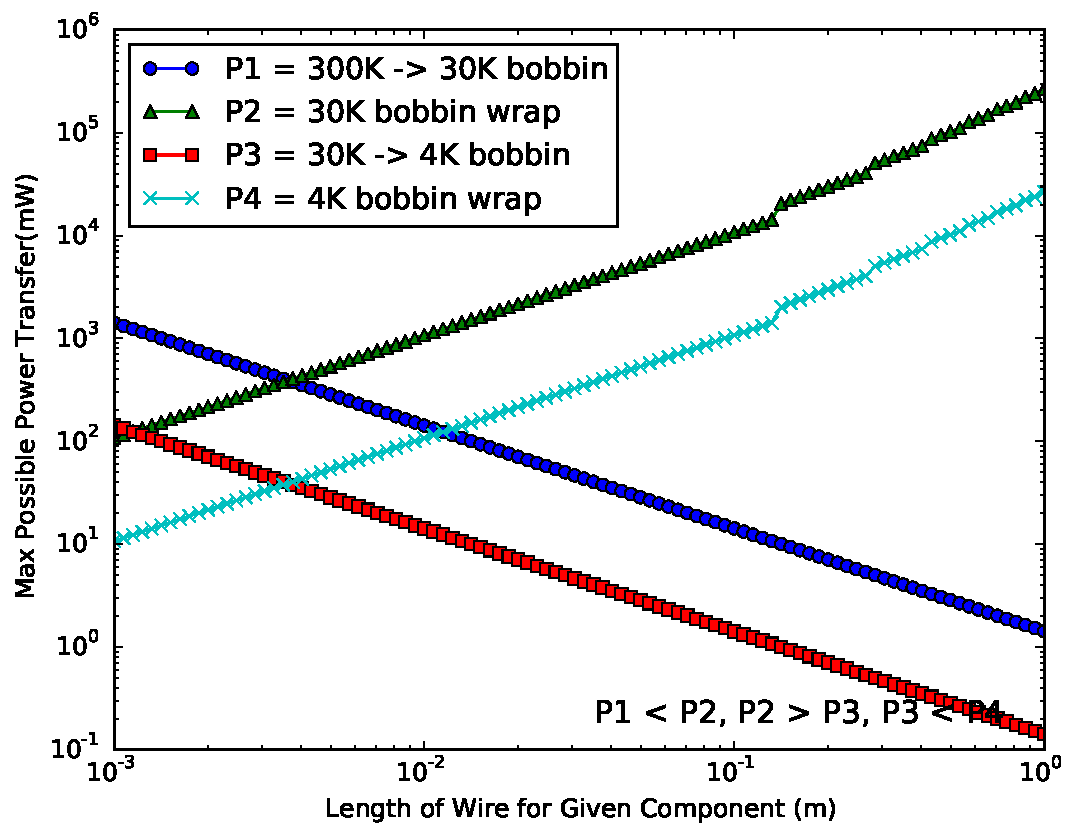
\includegraphics[width=\columnwidth]{powertransver_vs_wirelen_forbobbins.pdf}
\caption{Power Transfer or Dissipated for each component.  The powers are all
multiplied by 50 to simulate 50 wires being brought into the cold}
\label{fig}
\end{figure}

First, note that the bobbin wraps positively sloped.  
This makes sense because the 
more you wrap the wires around the bobbin, the more heat the bobbin can take 
away from the wires.  Similarly, the slope of the lengths of wire is negative
as the longer wires will not transfer as much power to the cold.  On the 
bobbin wraps, note the little steps at high wire length.  This is because when
one starts wrapping in different layers, weird things start happening.  
%TODO
\textbf{TODO: I'm
not sure about this... I think it should step down a little.  I'll have to look
more into this.}
However, this is not essential to our dialog, as the difference is very small.

Looking at the levels of the plots, we can see that \(P_1<P_2\) after 
\(3\units{mm}\) of each wire.  We know that \(P_1\) should have at least 
\(10 \units{cm}\) of wire just by geometry of our measurement setup so that 
puts us in a safe region.  Then, we note that for \(P_3 < P_4\) we need about 
\(3\units{mm}\).  Again, this is not a problem.  The bobbins will probably
have centimeters of wire around them.  We are home free in power transfer.  
That means that bobbins with stycast with a few turns (\(<10\) centimeter of 
total wire length around the bobbin) will be sufficient to thermalize the wires.

Lets consider the heat load at \(4K\).  Our goal is to limit the heat as much 
we can.  We see that any heat load will not be from 300K, but from 30K.  So, we 
need to make the wires from the 30K to 4K long.  Wires \(\sim 1\units{cm}\) will
give \(10 \units{mW}\) of heating, wires \(\sim 10 \units{cm}\) will give us
\(2 \units{mW}\) of heating.  The bobbin at the 4K stage is pretty 
inconsequential when the power flowing into 4K is so low.

\section{Conclusion}
I did a preliminary model of power transfer into the montana cryostat and found
that we do not need that much wire.  If we get a few good loops around the 
bobbins, they should thermalize properly.  However, to limit power transfer to
4K, we need to make the wires from the 30K to 4K stage long.  

Also, it is never bad to make the 300K to 30K wires longer, as that will
probably improve our base temperature as it will limit the amount of cooling
power required at 30K.  
\end{document}
